\documentclass[10pt,a4paper,twoside,openright,titlepage,twocolumn]{article}
\usepackage[utf8]{inputenc}
\usepackage[T1]{fontenc}
\usepackage{amsmath}
\usepackage{amssymb}
\usepackage{graphicx}
\usepackage{xcolor}
\usepackage{wrapfig}
\usepackage{siunitx}
\usepackage{titlesec}
\usepackage{titlepic}
\usepackage[export]{adjustbox}
\usepackage[left=6.00mm, right=6.00mm, top=6.00mm, bottom=12.00mm]{geometry}
\usepackage{listings}

\graphicspath{ {./Images/} }

\definecolor{formulablue}{RGB}{219,219,255}
\newcommand{\formula}[1]{\colorbox{formulablue}{#1}}

\newcommand{\unitText}[3]{\noindent\textit{#1} : #2 [#3]}

\definecolor{refrot}{RGB}{183,28,42}
\definecolor{LightGray}{gray}{0.9}
\definecolor{ForestGreen}{RGB}{34,139,34}
\newcommand{\refskript}[1]{\textcolor{refrot}{#1}}
\newcommand{\refskriptP}[1]{\textcolor{refrot}{Skript S.#1}}

% Setup Source Code
\lstset{ 
	backgroundcolor=\color{white},   % choose the background color; you must add \usepackage{color} or \usepackage{xcolor}; should come as last argument
	basicstyle=\footnotesize,        % the size of the fonts that are used for the code
	breakatwhitespace=true,         % sets if automatic breaks should only happen at whitespace
	breaklines=true,                 % sets automatic line breaking
	captionpos=b,                    % sets the caption-position to bottom
	commentstyle=\color{ForestGreen},    % comment style
	escapeinside={\%*}{*)},          % if you want to add LaTeX within your code
	extendedchars=true,              % lets you use non-ASCII characters; for 8-bits encodings only, does not work with UTF-8
	frame=single,	                   % adds a frame around the code
	keepspaces=true,                 % keeps spaces in text, useful for keeping indentation of code (possibly needs columns=flexible)
	language=C,                      % the language of the code
	numbersep=5pt,                   % how far the line-numbers are from the code
	rulecolor=\color{black},         % if not set, the frame-color may be changed on line-breaks within not-black text (e.g. comments (green here))
	showspaces=false,                % show spaces everywhere adding particular underscores; it overrides 'showstringspaces'
	showstringspaces=false,          % underline spaces within strings only
	showtabs=false,                  % show tabs within strings adding particular underscores
	stepnumber=2,                    % the step between two line-numbers. If it's 1, each line will be numbered
	tabsize=2,	                   % sets default tabsize to 2 spaces
	title=\lstname,                   % show the filename of files included with \lstinputlisting; also try caption instead of title
	stringstyle=\ttfamily\color{red!50!brown},
	keywordstyle=\color{blue}\bfseries,
	literate={~} {$\sim$}{1}
}

\setlength{\parindent}{0pt}

\titlespacing*{\section}{0pt}{12pt}{0pt}
\titlespacing*{\subsection}{0pt}{0pt}{0pt}
\titlespacing*{\subsubsection}{0pt}{0pt}{0pt}

\title{\vspace{50mm}SigSys2 \\ [1ex] \large Formelsammlung}
\author{Sebastian Humbel}
\titlepic{\vspace{50mm}
\includegraphics[width=0.25\textwidth]{Elvis}}




\begin{document}
	\maketitle
	%\section{Section1}
\subsection{Subsection1}
\begin{minipage}[t]{0.3\textwidth}
	\vspace{0pt}								% Abbildung hier einfügen
	\includegraphics[width=\textwidth]{"Bild"}
\end{minipage}\hspace{0.05\textwidth}
\begin{minipage}[t]{0.65\textwidth}
	\vspace{0pt}								% Beschreibung und Formeln hier einfügen
	Beschreibung zum Thema. \refskript{10}\\
	\formula{$1+1 = 2$}
	\formula{$1+1 = 2$}
\end{minipage}
\vspace{2mm}

\noindent
\begin{minipage}{0.5\textwidth}
	\unitText{Symbol}{Beschreibung}{$Einheit$}
\end{minipage}%%%
\begin{minipage}{0.5\textwidth}
	\unitText{Symbol}{Beschreibung}{$Einheit$}
\end{minipage}




\section{Section2}
\subsection{Subsection2}
\begin{minipage}[t]{0.3\textwidth}
	\vspace{0pt}								% Abbildung hier einfügen
	\includegraphics[width=\textwidth]{"Bild"}
\end{minipage}\hspace{0.05\textwidth}
\begin{minipage}[t]{0.3\textwidth}
	\vspace{0pt}								% Beschreibung und Formel hier einfügen
	Beschreibung zum Thema und ein Test wie breit
	man schreiben kann. \refskript{10}\\
	\begin{center}
		\formula{$1+1 = 2$}\\
		\formula{$\sum{3a+x}$}
	\end{center}
\end{minipage}\hspace{0.05\textwidth}
\begin{minipage}[t]{0.3\textwidth}
	\vspace{0pt}								% Einheiten hier einfügen
	\unitText{Symbol}{Beschreibung}{$Einheit$}
\end{minipage}




	\section{GPIO \refskript{8.1, 8.2}}


	\section{Interrupt Concepts \refskript{7.1, 7.2}}
A Interrupt is a signal indicating the occurrence of an event that needs immediate CPU attention.
There exist different types of Interrupts:
\begin{itemize}
	\itemsep-.5em 
	\item Hardware triggers
	\item Software triggers
	\item CPU exceptions
\end{itemize}

\begin{lstlisting}[language=c]
PxDIR &= ~0x01;	// Set Px.0 as input
PxDIR |=  0x02;	// Set Px.1 as output
PxOUT &= ~0x02;	// Clear LED on Px.1
PxIE  |=  0x01;	// IRQ when SW1 is pressed
...
__interrupt void portx_ISR(void) {
	PxOUT ^=  0x02;
}
\end{lstlisting}\vspace{-25px}

\subsection{Maskabe vs. Nonmaskable \refskript{7.1.2}}
\textit{Maksable}: Can be blocked (masked), trough flags. Most common type of interrupt. Disabled upon RESET.

\textit{Non-maskable} interrupts (NMI): Cannot be masked, thus are always served. Reserved for system critical events

Also see \refskript{7.2.2} and \refskript{7.2.3}


\subsubsection{Interrupt Flow}
\includegraphics[width=.6\columnwidth, center]{"InterruptFlow"}

Interrupt kann über intrinsische Funktionen eingestellt werden.
Alternativ mit enable\_interrupt() funktion.


\subsubsection{Interrupt Service Sequence \refskript{7.1.3}}
PC speicher den aktuellen ort im code bevor der Interrupt ausgeführ wird.
SR wird auf dem stack gespeichert

\subsubsection{Interrupt Identification Methods \refskript{7.1.4}}
\textit{Non-vectored systems (1)} don't know, what triggered the interrupt and have to identify the interrupt source within the ISR.

\textit{Vectored interrupts (2)} Have an ID for each interrupt type an can jump directly to the desired ISR.

\textit{Auto-vectored interrupts (3)} have predefined addresses / fix vectors for the different interrupts.

\subsubsection{Interrupt Priority Handling \refskript{7.1.5}}
(1) \textit{Polling order of SRQ flags} decides priority (if else if define the interrupt priority)

(2) \textit{Daisy Chain-based Arbitration} defines the priority through hardwired logic. Used by the MSP430.

(3) \textit{Interrupt controller-based Arbitration} allows priority configuration by the user.

\subsection{Interrupt Software Design \refskript{7.3}}
\begin{lstlisting}[language=c]
// main.c
int main(void){
	hal_gpio_init();
	hal_gpio_interruptCallbackFctRegister(
					GPIO_S1,_s1_callbackFct);
}

static void _s1_callbackFct(void){
	...
}
\end{lstlisting}\vspace{-25px}
\begin{lstlisting}[language=c]
// hal_gpio.h
void hal_gpio_init(void);
void hal_gpio_interruptCallbackFctRegister(
			gpioPeripherie_t gpio, pFctHandler pCallbackFct);
\end{lstlisting}\vspace{-25px}
\begin{lstlisting}[language=c]
// hal_gpio.c
void hal_gpio_init(void) { // ... }
void hal_gpio_interruptCallbackFctRegister(
		gpioPeripherie_t gpio, pFctHandler pCallbackFct) {
			_hal_gpio_callbackFct[0] = pCallbackFct;
}

#pragma vector=PORT1_VECTOR
__interrupt void _port1_ISR(void) {
	// ...
	_hal_gpio_callbackFct[0](); // call back application code
}
\end{lstlisting}\vspace{-25px}




	\section{Clock System}
\subsection{Clock Sources \refskript{6.3}}
Clock settings in \textit{CSCTL} register.\\
Voltage Swing $V_{SW} = V_{OH} - V_{OL}$ : Amplitude from low to high.\\
Frequency $f_{clk} = \dfrac{1}{T_{clk}}$ : Number of cycles per second\\
Duty Cycle $DC = \dfrac{t_{high}}{T_{clk}} * 100 \%$ : Ratio of high time to period\\
Edge Speed $t$ and $t_f$ : Rising and falling times

\includegraphics[width=\columnwidth]{"clock"}

\subsection{Clock Stability \refskript{6.3.1}}
Statistical measure of the maximum allowable parameter fluctuations of a clock signal
over a given time interval.

\begin{minipage}[t]{0.5\columnwidth}
	Possible factors:
	\begin{itemize}
		\itemsep-.5em 
		\item type of oscillator
		\item capacitive load
		\item ageing
		\item supply voltage or temperature
	\end{itemize}
\end{minipage}
\begin{minipage}[t]{0.5\columnwidth}
	Short- and long-term effects:
	\begin{itemize}
		\itemsep-.5em 
		\item Clock Jitter
		\item Clock Drift
	\end{itemize}
\end{minipage}
\vspace{2mm}

\subsection{Source Selection \refskript{6.3.2}}
Choose the lowest frequency that allows for a reliable and correct system operation.
Adjust the frequency to the speed of the fastest event.


\subsection{Internal vs. External Clock \refskript{6.3.3}}

\begin{minipage}[t]{0.5\columnwidth}
	\textbf{Internal}
	
	Pro:
	\begin{itemize}
		\itemsep-.5em 
		\item Reduce external component count
		\item Less expensive
		\item Induce lower power consumption
	\end{itemize}
	Con:
	\begin{itemize}
		\itemsep-.5em 
		\item Reduced clock stability
		\item Less flexibility
		\item Narrower bandwidth
	\end{itemize}
\end{minipage}
\begin{minipage}[t]{0.5\columnwidth}
	\textbf{External}
	
	Pro:
	\begin{itemize}
		\itemsep-.5em 
		\item Wider choice of frequencies
		\item More design flexibility
	\end{itemize}
	Con:
	\begin{itemize}
		\itemsep-.5em 
		\item Increment the external component count
		\item Higher clock speeds induce higher power
		consumption
	\end{itemize}
\end{minipage}
\vspace{2mm}

\subsection{RC-based Oscillator}
\includegraphics[width=0.7\columnwidth, center]{"rcbased_oscillator"}

\subsection{Quartz Crystal Oscillators \refskript{6.3.4}}
Based on mechanical resonance of a vibrating piezoelectric crystal.

\subsection{Pierce Crystal Oscillator \refskript{6.3.4}}
Series Resonant Oscillator

\subsection{Colpitts Crystal Oscillator \refskript{6.3.4}}
Parallel Resonant Oscillator

\subsection{Oscillator Startup Time \refskript{6.3.4}}

\section{The MSP430 System Clock \refskript{6.4}}
\includegraphics[width=0.7\columnwidth, center]{"MSP430clocksystem"}

\subsection{DCO Clock}
Digitally controlled oscillator
\begin{enumerate}
	\itemsep-.5em 
	\item Select a frequency range (DCORSEL)
	\item Select the frequency within that range (DCO)
	\item Setup Modulation (MOD)
\end{enumerate}
\includegraphics[width=0.5\columnwidth]{"DCOwide"}
\includegraphics[width=0.5\columnwidth]{"DCOnarrow"}

\includegraphics[width=0.5\columnwidth]{"DCOmod1"}
\includegraphics[width=0.5\columnwidth]{"DCOmod2"}









	\section{Timer \& Event Counters \refskript{7.4}}
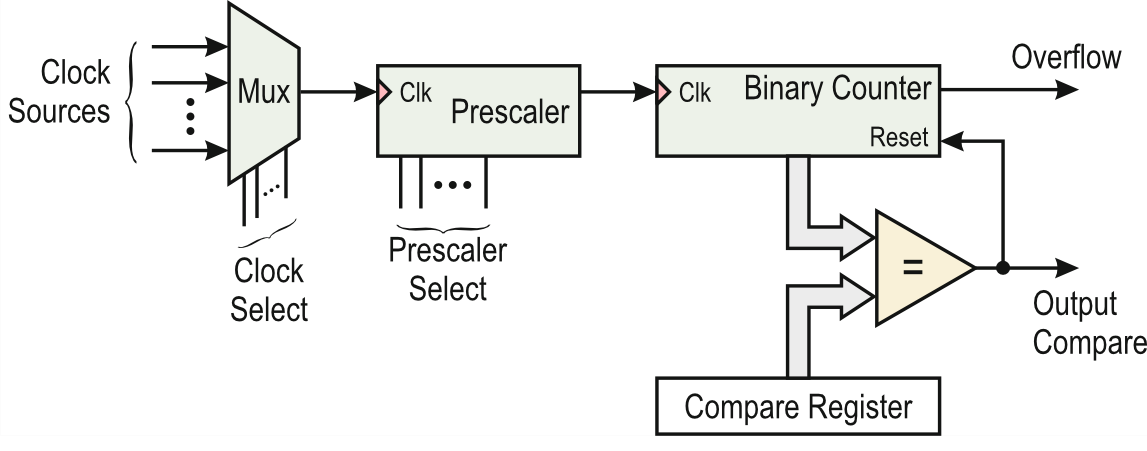
\includegraphics[width=\columnwidth]{"Images/TimerFuntionsweise.png"}

\subsection{Signature Timer Applications \refskript{7.4.3}}
\textit{Watchdog timer} is secured through a password in the \textit{WDTCTL} register.
\textit{Real-Time Clocks} provides absolute time (second, minute, hour, day, month, week).
\textit{Baud Rate Generation} can provide clock base for baud rate.

\begin{minipage}{.5\columnwidth}
	\formula{$\mathit{baudrate} = \dfrac{f_{\mathit{clk}}}{\mathit{PS} \cdot \mathit{TopCount}}$}
\end{minipage}
\begin{minipage}{.5\columnwidth}
	\unitText{$\mathit{PS}$}{Prescale Factor}{1}\\
	\unitText{$f_{\mathit{clk}}$}{Clock frequency}{Hz}\\
	\unitText{$\mathit{TopCount}$}{Compare value}{1}
\end{minipage}

\subsubsection{MSP430 Timer Support \refskript{7.4.4}}

Operating Modes

Input Capture Operation

Measuring a Signal Width

Output Compare Operation
	\section{Low-Power Modes \refskript{7.3.6}}
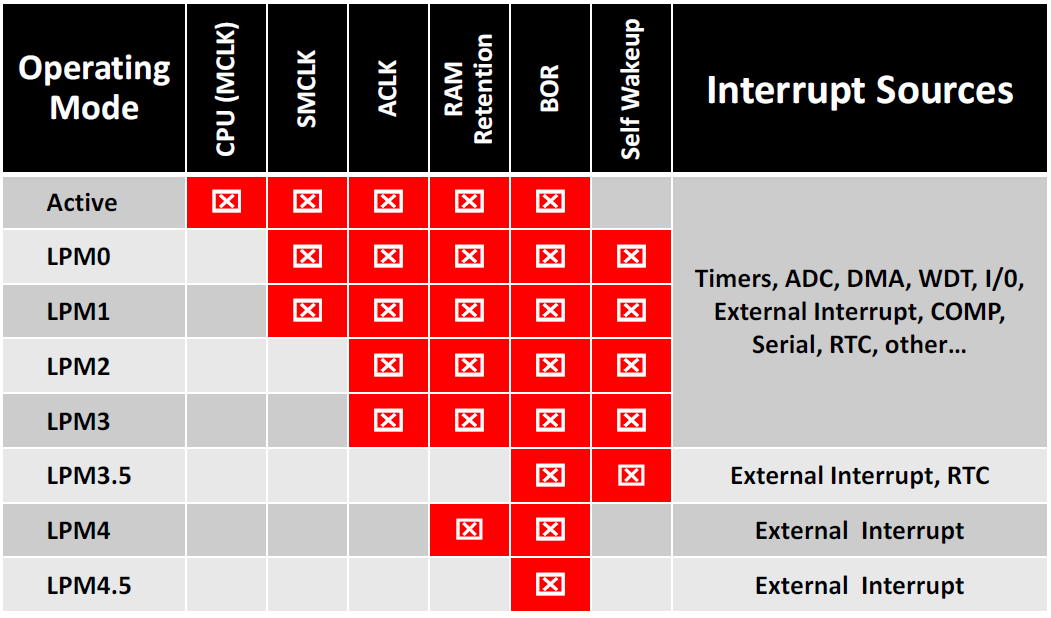
\includegraphics[width=.8\columnwidth, center]{Images/LPO_interrupts.png}

\subsection{Activity Profiles}

\subsection{Power Consumption in CMOS Technology}
\begin{minipage}{0.5\columnwidth}
	\vspace{0pt}
	\formula{$P \sim \alpha C_L V_{dd}^2 f$}
	\formula{$E \sim  \alpha C_L V_{dd}^2 f t$}
	\formula{$E \sim \alpha C_L V_{dd}^2 \mathit{(\# cycles)}$}
	
	\formula{$\tau \sim C_L \dfrac{V_dd}{(V_dd - V_T)^2}$}
	\formula{$f \sim \dfrac{1}{\tau} \sim V_{dd}$}
\end{minipage}
\begin{minipage}{0.5\columnwidth}
	\vspace{0pt}
	\unitText{$V_{dd}$}{supply voltage}{\unit{V}}\\
	\unitText{$V_T$}{threshold voltage}{\unit{V}}
	\unitText{$\alpha$}{switching activity}{\unit{1}}\\
	\unitText{$C_L$}{load capacity}{\unit{F}}\\
	\unitText{$f$}{clock frequency}{\unit{Hz}}\\
	\unitText{$\tau$}{Gate delay}{\unit{ms}}
\end{minipage}
\vspace{2mm}


\subsection{Interrupts and Low-Power Modes}
Low power modes are configured with the bits \textit{CPUOFF}, \textit{OSCOFF}, \textit{SCG0} and \textit{SCG1} in the \textbf{Status Register} (SR, also called R2).

\subsection{CCS6 Intrinsic Functions for MSP430}
\begin{lstlisting}[language=c]
	#include <intrinsics.h>
\end{lstlisting}

\subsection{Low-Power Optimization}
Replace software with hardware peripherals.
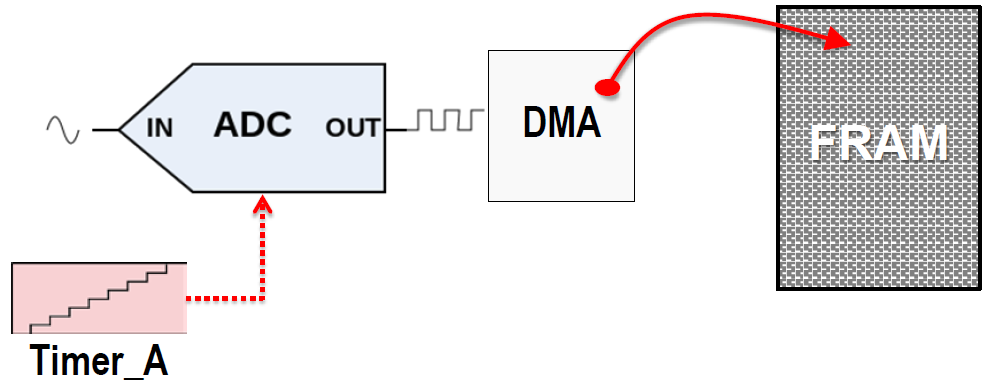
\includegraphics[width=0.8\columnwidth, center]{Images/LPM_replace_hw_with_sw.png}

\section{Real-Time Clock (RTC) \refskript{7.4.3}}
\subsection{RTC Interrupts}
\begin{enumerate}
	\itemsep-.5em 
	\item Alarm
	\item Interval Timer
	\item Prescaler 0
	\item Prescaler 1
	\item Ready for Register operation
\end{enumerate}

Example 1: Time Event
\begin{lstlisting}[language=C]
int main (void)
{
	WDTCTL = WDTPW | WDTHOLD;	//stop watchdog
	//disable high-impedance ports
	PM5CTL0 &= ~LOCKLPM5;
	//just for testing (P1.0 / LED1)
	P1DIR |= 0x01;
	P1OUT &= ~0x01;
	
	PJSEL0 = BIT4 | BIT5; //Init. LFXT pins
		
	//Configure LFXT 32kHz crystal
	CSCTL0_H = CSKEY >> 8;	//Unlock CS reg.
	CSCTL4 &= ~LFXTOFF;			//Enable LFXT
	do
	{
		//Clear LFXT fault flag
		CSCTL5 &= ~LFXTOFFG;
		SFRIFG1 &= ~OFIFG;
		//Test oscillator fault flag
	} while (SFRIFG1 & OFIFG);
	CSCTL0_H = 0;	//Lock CS registers
		
	//write RTCKEY to unlock RTC reg. for write
	RTCCTL0_H = 0xA5;
	//hold RTC, clock from output of RT1PS,
	// RTCTEVIFG on 8-bit overflow
	RTCCTL1 = 0x48;
		
	//Enable time event interrupt
	RTCCTL0_L = 0x40;
	//prescale timer 0: divided by 64
	RTCPS0CTL = 0x2800;
	//prescale timer 1: out from RT0PS, div. by 2
	RTCPS1CTL = 0x8000;
	//Enable RTC
	RTCCTL1 &= ~0x40;
	//Enter LPM3 with interrupt enabled
	__bis_SR_register(LPM3_bits + GIE);
		
	while (1)
	{}
}
\end{lstlisting}

Example 2: RTC Calendar
\begin{lstlisting}[language=C]
//BCD, hold RTC, RTCMode, one minute overflow
RTCCTL1 = 0xE0;

RTCSEC = 0x00;	//Set Seconds
RTCMIN = 0x00;	//Set Minutes
RTCHOUR = 0x10;	//Set Hours
RTCDOW = 0x03;	//Set DOW (sunday = 0)
RTCDAY = 0x18;	//Set Day
RTCMON = 0x10;	//Set Month
RTCYEAR = 0x2023;	//Set Year

//setup alarm
//enable minutes alarm, minutes = 1 and others are don't care
// --> so an alarm is generated on 00:01:00, 01:01:00, ...
RTCAMIN = 0x81;
RTCAHOUR = 0x00;
RTCADOW = 0x00;
RTCADAY = 0x01;

RTCCTL0_L = 0x60;
//Enable time event & alarm interrupt
RTCCTL1 &= ~0x40;
//Enable RTC
__bis_SR_register(LPM3_bits + GIE); //Enter LPM3 w/ interrupt
while (1)
{}
\end{lstlisting}





\end{document}


